\documentclass{BHCexam}
\usepackage{yhmath}%弧度表示
\newcommand{\xl}[2]{\vv{#1}\bm\cdot\vv{#2}}
\begin{document}
\newtheorem{Theroem}{定理}
\biaoti{向量}
\fubiaoti{}
\maketitle
\setcounter{tocdepth}{2}
\tableofcontents
\newpage 
\section{基本概念}
\begin{description}
\item[向量] 既有大小,又有方向的量,用$ \vv{a},~\vv{AB},~\bm{a} $表示;向量的大小叫做向量的模,用$ \abs{\bm{a}} $表示.\par
{\kaishu 平面向量是自由向量(无源向量).此文后面不加说明一般用黑体$ \bm{a} $表示向量}
\item[零向量] 长度为零的向量,其方向是任意的,记作$ \vv{0} $或$ \bm{0} $;
\item[单位向量] 长度等于一个单位长度的向量;
\item[平行向量(共线向量)]方向相同或相反的非零向量叫做平行向量或共线向量;$ \bm{0} $与任一向量共线;
\item[相等向量] 长度相等且方向相同的向量;\par
{\kaishu 两个向量只能相等或者不相等,不能比较大小.}
\item[相反向量] 长度相等且方向相反的向量
\end{description}
\section{向量的线性运算}
\subsection{加法}
\begin{description}
\item[定义] 两个向量和的运算;
\item[法则] 平行四边形法则或三角形法则
\begin{center}
\begin{tikzpicture}
\coordinate(O) at (0,0);
\coordinate(A) at (2,0);
\coordinate(B) at(1,2);
\coordinate(C) at ($(A)+(B)$);
\draw[->,>=latex] (O)--(A)node[midway,below](a){\small$\bm{a}$};
\draw[->,>=latex] (O)--(C)node[midway,above,sloped](a){\small$\bm{a}+\bm{b}$};
\draw[->,>=latex] (A)--(C)node[midway, below](a){\small$\bm{b}$};
\begin{scope}[xshift=4cm]
\coordinate(O) at (0,0);
\coordinate(A) at (2,0);
\coordinate(B) at(1,2);
\coordinate(C) at ($(A)+(B)$);
\draw[->,>=latex] (O)--(A)node[midway ,below](a){\small$\bm{a}$};
\draw[->,>=latex] (O)--(C)node[midway ,below,sloped](a){\small$\bm{a}+\bm{b}$};
\draw[->,>=latex] (O)--(B)node[midway, left](a){\small$\bm{b}$};
\draw[dashed](B)--(C);
\draw[dashed](A)--(C);
\end{scope}
\end{tikzpicture}
\end{center}
\item[坐标表示] 给定向量$ \bm{a}=(x_1,y_1),~\bm{b}=(x_2,y_2) $.有:\[\bm{a}+\bm{b}=(x_1+x_2,y_1+y_2)\]
\end{description}
\subsection{减法}
\begin{description}
\item[定义]求$ \bm{a} $与$\bm{b}$的相反向量$-\bm{b}$的和的运算叫做$\bm{a}$与$\bm{b}$的差
\item[运算法则]三角形法则、平行四边形法则,$\vv{AB}-\vv{AC}=\vv{CB}$.
\begin{center}
\begin{tikzpicture}
\coordinate(O) at (0,0);
\coordinate(A) at (2,0);
\coordinate(B) at(1.5,1.5);
\draw[->,>=latex] (O)--(A)node[midway,below](a){\small$\bm{b}$};
\draw[->,>=latex] (O)--(B)node[midway, left](a){\small$\bm{a}$};
\draw[->,>=latex](A)--(B)node[midway, above,sloped](a){\small$\bm{a}-\bm{b}$};
\begin{scope}[xshift=6cm]
\coordinate(O) at (0,0);
\coordinate(B) at (2,0);
\coordinate(A) at(1.5,1.5);
\coordinate(B1) at (-2,0);
\coordinate(C)at($(B1)+(A)$);
\draw[->,>=latex] (O)--(B)node[midway,below](a){\small$\bm{b}$};
\draw[->,>=latex] (O)--(A)node[midway, left](a){\small$\bm{a}$};
\draw[->,>=latex](B)--(A)node[midway, above,sloped](a){\small$\bm{a}-\bm{b}$};
\draw[->,>=latex](O)--(B1)node[midway,below](b1){\small$\bm{-b}$};
\draw[->,>=latex](O)--(C)node[midway,below,sloped](b1){\small$\bm{a-b}$};
\draw[dashed] (B1)--(C) (A)--(C);
\end{scope}
\end{tikzpicture}
\end{center}
\item[坐标表示] 给定向量$ \bm{a}=(x_1,y_1),~\bm{b}=(x_2,y_2) $.有:\[\bm{a}-\bm{b}=(x_1-x_2,y_1-y_2)\]
\end{description}
\subsection{数乘}
\begin{description}
\item[定义] 求实数$ \lambda $与向量$\bm{a}$的积的运算
\item[法则]\begin{enumerate}[1)]
\item $ \abs{\lambda \bm{a}}=\abs{\lambda}\abs{\bm{a}} $;
\item 当$ \lambda>0 $时,$ \lambda\bm{a} $的方向与$\bm{a}$的方向相同;
\item 当$ \lambda<0 $时,$ \lambda\bm{a} $的方向与$\bm{a}$的方向相反;
\end{enumerate}
\end{description}
\begin{Theroem}[向量共线定理]
向量$\bm{a}~(\bm{a}\ne\bm{0})$与向量$\bm{b}$共线的充要条件是存在唯一的实数$ \lambda $,使得$\bm{b}=\lambda\bm{a}$.
\end{Theroem}
\section{平面向量基本定理及坐标表示}
\subsection{基底}
\begin{Theroem}[平面向量基本定理]
如果$ \bm{e}_1,\bm{e}_2 $是同一平面内的两个\CJKunderdot{不共线}的向量,那么对于这一平面内的任意向量$ \bm{a} $,有且只有一对实数$ \lambda_1,~\lambda_2 $,使$\bm{a}=\lambda_1\bm{e}_1+\lambda_2\bm{e}_2$.\par 其中,不共线的向量$ \bm{e}_1,~\bm{e}_2 $叫做表示这一平面内所有向量的一组\CJKunderdot{基底}.
\end{Theroem}
{\kaishu 解决向量问题,需要注意两点:一是向量共线定理,一个是平面向量基本定理.\par
向量的基底的重要性在于一旦有了基底,你就可以将题目中涉及的所有向量都用基底向量唯一的表示出来(坐标表示就是一组特殊的基底),计算和变形都有了方向,便于寻找和发现关系.如果题目没有明确给出基底,那么就需要自己指定了}

\subsection{坐标表示}
在不共线的向量中,垂直是一种重要的情形,把一个向量分解为两个互相垂直的向量,叫做把向量\CJKunderdot{正交分解}.\par
在平面直角坐标系$xOy$中,分别取与$x$轴、$y$轴方向相同的两个\CJKunderdot{单位向量}$~ \bm{i},~\bm{j} $作为基底.对于平面内的一个向量$ \bm{a} $,由平面向量基本定理可知,有且只有一对实数$ x,~y $使得\[\bm{a}=x\bm{i}+y\bm{j}\]
这样,平面内的任一向量$ \bm{a} $都可以由$ x,~y $唯一确定,我们把有序数对$ (x,y) $叫做向量$\bm{a}  $的坐标,记作\begin{equation}\label{axy}
\bm{a}=(x,y)
\end{equation}其中$ x $叫做$ \bm{a} $在$x$轴上的坐标,其中$ y $叫做$ \bm{a} $在$y$轴上的坐标,(\ref{axy})式叫做\textbf{向量的坐标表示}
\begin{center}
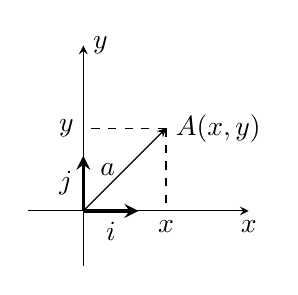
\begin{tikzpicture}[scale=0.7]
\draw[->,>=stealth] (-1,0)--(3,0) node[below](x){$x$};
\draw[->,>=stealth] (0,-1)--(0,3) node[right](y){$y$};
\draw[very thick,->,>=stealth](0,0)--(1,0)node[midway,below](i) {$\bm{i}$};
\draw[very thick,->,>=stealth](0,0)--(0,1)node[midway,left](j) {$\bm{j}$};
\coordinate(A) at (1.5,1.5);
\node[right](a1)at(1.5,1.5){$A(x,y)$};
\draw[dashed](A)--++(-1.5,0)node[left](y){$y$};
\draw[dashed](A)--++(0,-1.5)node[below](x){$x$};
\draw[->,>=stealth](0,0)--(A) node[midway,left] (a) {$\bm{a}$};
 \end{tikzpicture}
\end{center}

\begin{description}
\item[三点共线的判定] 若$ A,~B,~C $三点共线,有$ \vv{OA}=\lambda \vv{OB}+\mu\vv{OC}~(\lambda+\mu=1) $.或$\vv{AB}=\lambda \vv{AC}$.
%\begin{enumerate}[1)]
%
%\end{enumerate}
\end{description}
\subsection{平面向量的坐标计算}
\begin{enumerate}
\item  设点$ A(x_1,y_1),~B(x_2,y_2) $,则$ \vv{AB}=(x_2-x_1,y_2-y_1) $.\par 
一个向量的坐标等于表示此向量的有向线段的终点的坐标减去起始点的坐标.
\item 若$\bm{a}=\left(x_1,y_1\right),\bm{b}=\left(x_2,y_2\right)$.
\begin{description}
\item[加法:] $\bm{a}+\bm{b}=(x_1+x_2,y_1+y_2)$
\begin{equation*}
\begin{aligned}
\bm{a}+\bm{b}=&\left(x_1\bm{i}+y_1\bm{j}\right)\left(x_2\bm{i}+y_2\bm{j}\right)\\
=&\left(x_1+x_2\right)\bm{i}+\left(y_1+y_2\right)\bm{j}\\
\text{即:}\bm{a}+\bm{b}=&(x_1+x_2,y_1+y_2)
\end{aligned}
\end{equation*}
\item[减法:] $\bm{a}-\bm{b}=\left(x_1-x_2,y_1-y_2\right)$.同加法可得
\item[数乘:] $ \lambda \bm{a}=\left(\lambda x_1,\lambda y_1\right) $\begin{equation*}
\begin{aligned}
 \lambda \bm{a} =&\lambda\left(x_1\bm{i}+y_1\bm{j}\right)=\lambda x_1\bm{i}+\lambda y_1\bm{j}\\
=&\left(\lambda x_1,\lambda y_1\right)
\end{aligned}
\end{equation*}

\item[模长]
 $\abs{\bm{a}}=\sqrt{x_1^2+y_1^2}$\qquad
 $\abs{\vv{AB}}=\sqrt{(x_2-x_1)^2+(y_2-y_1)^2}$\\
\qquad $\abs{\bm{a}+\bm{b}}=\sqrt{(\bm{a}+\bm{b})^2}=\sqrt{\bm{a}^2+2\bm{a}\bm{\cdot}\bm{b}+\bm{b}^2}$\\

\item[共线] 由向量共线的性质知$ \bm{a} $与$ \bm{b}(\bm{b}\ne\bm{0}) $共线,当且仅当存在实数$ \lambda $使得$ \bm{a}=\lambda \bm{b} .$\\用坐标表示为:
$$(x_1,y_1)=\lambda(x_2,y_2)$$
即$$\Bigg\{\begin{aligned}
x_1=&\lambda x_2\\
y_1=&\lambda y_2
\end{aligned}$$
消去$ \lambda $得到\[x_1y_2-x_2y_1=0\]
\item[垂直] $\bm{a}\bm{\bot}\bm{b}\Leftrightarrow\bm{a}\bm{\cdot}\bm{b}=0\Leftrightarrow x_1x_2+y_1y_2=0 $
\begin{proof}
\begin{description}
\item[方法一]设$ \bm{a},~\bm{b} $所在直线分别为$ l_1,l_2 $,当$ \bm{a},~\bm{b} $所在直线的斜率都存在时,由直线垂直的性质,有$$ k_{l_1}\bm{\cdot}k_{l_2}=-1 $$ 
其中$$ k_{l_1} =\dfrac{y_1-0}{x_1-0}=\dfrac{y_1}{x_1},\quad k_{l_2} =\dfrac{y_2-0}{x_2-0}=\dfrac{y_2}{x_2}$$
即$$\dfrac{y_1}{x_1}\bm{\cdot}\dfrac{y_2}{x_2}=-1$$
$$x_1x_2+y_1y_2=0$$
\item[方法二] 由向量的数量积性质,当$ \bm{a}\bot\bm{b} $时,
$\text{由}\cos\theta=\dfrac{\bm{a\cdot b}}{\abs{\bm{a}}\abs{\bm{b}}}\text{得到}$\\
\centering $\bm{a\cdot b}=0$
\end{description}
\end{proof}

\end{description}
\end{enumerate}


\section{平面向量的数量积}
\subsection{定义}
\begin{description}
\item[定义] 已知两个非零向量$ \bm{a} $与$\bm{b}$,我们把数量$ \abs{\bm{a}}\abs{\bm{b}}\cos\theta $叫做$ \bm{a} $与$ \bm{b} $的数量积(\textbf{内积}),记作$ \bm{a}\bm{\cdot}\bm{b} $,即\[\bm{a}\bm{\cdot}\bm{b}=\abs{\bm{a}}\abs{\bm{b}}\cos\theta\]
其中$ \theta $为$ \bm{a} $与$ \bm{b} $的夹角.
\item[几何意义] 数量积$ \bm{a}\bm{\cdot}\bm{b} $等于$\bm{a} $的模长$ \abs{\bm{a}} $与$ \bm{b} $在$ \bm{a} $的方向上的投影$ \abs{\bm{b}}\cos \theta $的乘积.\par 
{\kaishu \textbf{注:}当$ \theta=0 $时,$ \cos\theta=1 $,所以有$ \bm{a\cdot b}=\bm{\abs{a}\abs{b}} $;\\\phantom{注:\ }当$ \theta=90^{\circ} $时,有$ \cos\theta =0$,所以有$ \bm{a\cdot b}=0 $ \\\phantom{注:\ }当$ \theta=180^{\circ} $时,有$ \cos\theta =-1$,所以有$ \bm{a\cdot b}=-abs{\bm{a}}\abs{\bm{b}} $   }
\item[数量积计算] 
\begin{equation*}
\begin{aligned}
&\because \bm{a}=x_1\bm{i}+y_1\bm{j},~\bm{b}=x_2\bm{i}+y_2\bm{j},\\
&\therefore \bm{a}\bm{\cdot}\bm{b}=(x_1\bm{i}+y_1\bm{j})\bm{\cdot}(x_2\bm{i}+y_2\bm{j})\\
&\phantom{\therefore\bm{a}\bm{\cdot}\bm{b}~}=x_1x_2\bm{i}^2+x_1y_2\bm{i}\bm{\cdot}\bm{j}+x_2y_1\bm{i}\bm{\cdot}\bm{j}+y_1y_2\bm{j}^2.\\
& \bm{i}^2=\bm{j}^2=1,\bm{i}\bm{\cdot}\bm{j}=\bm{j}\bm{\cdot}\bm{i}=0\\
&\therefore \bm{a}\bm{\cdot}\bm{b}=x_1x_2+y_1y_2.
\end{aligned}
\end{equation*}

\item[夹角公式] $$ \cos\theta=\dfrac{\bm{a}\bm{\cdot}\bm{b}}{\abs{\bm{a}}\abs{\bm{b}}}=\dfrac{x_1x_2+y_1y_2}{\sqrt{x_1^2+y_1^2}\sqrt{x_2^2+y_2^2}} \quad \left(\theta\in\left[0,\pi\right],~\theta\text{也写作}\left<\bm{a},\bm{b}\right>\right).$$
\end{description}\par 
{\kaishu 直接求向量的数量积的方是近年高考的重点,其关键是根据向量的加减法则对向量进行基底分解.分解以后可以直接使用题目的已知条件,要么出现所要求的表达式(此时通过解一元一次方程).分解过程中,往往利用\CJKunderdot{垂直}将数量积消掉.\CJKunderdot{整体}的思想在数学中占据着极其重要的位置,求解整体的值时,往往不需要分别求出各个元素的值,而是将元素进行有效的分解、整合,提取有效的信息,从而求出整体的值.}
%\subsection{求向量夹角的方法}
%\begin{description}
%\item[坐标法] $\cos\theta=\dfrac{x_1x_2+y_1y_2}{\sqrt{x_1^2+y_1^2}\sqrt{x_2^2+y_2^2}}$
%\item[向量法] $\cos\theta=\dfrac{\bm{a}\bm{\cdot}\bm{b}}{\abs{\bm{a}}\abs{\bm{b}}}$
%\end{description}
\subsection{数量积相关补充}
\begin{enumerate}[(1)]
\item 若$\bm{a}=\left(x,y\right)$,则$ \bm{a}\bm{\cdot}\bm{a}=\bm{a}^2=\abs{\bm{a}}^2=x^2+y^2 $;
\item $ \abs{\bm{a}\pm \bm{b}}^2=\left(\bm{a}\pm \bm{b}\right)^2=\bm{a}^2\pm2\bm{a}\bm{\cdot}\bm{b}+\bm{b}^2 ;$
\item $\abs{\abs{\bm{a}}-\abs{\bm{b}}}\le\abs{\bm{a\pm b}}\le\abs{\bm{a}}+\abs{\bm{b}}$;
\item 若点$ A(x_1,y_1),~B(x_2,y_2) $,则$ \abs{\vv{AB}}=\sqrt{(x_2-x_1)^2+(y_2-y_1)^2} $;
\item \textbf{柯西-施瓦兹不等式:}若$\bm{a}=\left(x_1,y_1\right),\bm{b}=\left(x_2,y_2\right)$,则:$$ -\abs{\bm{a}}\abs{\bm{b}}\le\bm{a}\bm{\cdot}\bm{b}\le\abs{\bm{a}}\abs{\bm{b}}\Leftrightarrow -\sqrt{x_1^2+y_1^2}\sqrt{x_2^2+y_2^2}\le x_1x_2+y_1y_2\le \sqrt{x_1^2+y_1^2}\sqrt{x_2^2+y_2^2}$$
\item 若$ \abs{\bm{a}+\bm{b}}=\abs{\bm{a}-\bm{b}} $,则$ \bm{a}\bot\bm{b} $.对角线相等的平行四边形必然是矩形.
\item 若$ \left(\bm{a}+\bm{b}\right)\bm{\bot}\left(\bm{a}-\bm{b}\right) $,则$\abs{\bm{a}}=\abs{\bm{b}} $.对角线垂直的平行四边形必然是菱形.
\item 平面上$ O,~A,~B $三点不共线,设$\vv{OA}=\bm{a}=(x_1,y_1) ,~\vv{OB}=\bm{b}=(x_2,y_2)$,则$$ S_{\triangle OAB}=\dfrac{1}{2}\sqrt{\abs{\bm{a}}^2\abs{\bm{b}}^2-\left(\bm{a}\bm{\cdot}\bm{b}\right)^2}=\dfrac{1}{2}\abs{x_1y_2-x_2y_1} .$$
\item 给定两个长度为$ a $的平面向量$ \vv{OA},~\vv{OB} $,其夹角为$ \theta\in\left[0,\pi \right), ~$点$ C $在以$ O $为圆心的圆弧$ AB $上变动,若$ \vv{OC}=x\vv{OA}+y\vv{OB},~x,y\inR $,则$ x+y $的最大值为$ \sqrt{\dfrac{2}{\cos\theta+1}}. $
\end{enumerate}
\newpage 
\section{练习}
\begin{questions}

\qs
已知向量$ \vv{a}=(1,m),~\vv{b}=(3,-2) $,且$\left(\vv{a}+\vv{b}\right)\bot \vv{b} $,则$m$=\xx
\onech{$-8$}{$-6$}{$6$}{$8$}
\qs 若向量$ \bm{a,b,c} $满足$ \bm{a}\sslash\bm{b} $且$ \bm{a}\bot\bm{c} $,则$ \bm{c\cdot\left(a+2b\right)} =$\xx
\onech{$ 4$}{$ 3$}{$ 2$}{$ 0$}

\qs 若向量$ \bm{a,b} $满足:$ \abs{\bm{a}}=1,~\bm{\left(a+b\right)}\bot \bm{a},~\bm{\left(2a+b\right)}\bot \bm{b} $,~则$ \abs{\bm{b}}= $\xx
\onech{$ 2$}{$ \sqrt{2}$}{$ 1$}{$ \dfrac{\sqrt{2}}{2}$}
\qs 已知两个非零向量$\bm{ a,b}$满足$ \abs{\bm{a+b}}=\abs{\bm{a-b}} $,则下面结论正确的是\xx
\onech{$ \bm{a}\sslash \bm{b}$}{$ \bm{a}\bot\bm{b}$}{$\abs{\bm{a}}=\abs{\bm{b}} $}{$ \bm{a}+\bm{b}=\bm{a}-\bm{b}$}
\qs 若向量$ \bm{a} $与$ \bm{b} $不共线,$ \bm{a}\cdot \bm{b}\ne 0,~ $且$\bm{c}=\bm{a}-\left(\dfrac{\bm{a\cdot a}}{\bm{a\cdot b}}\right)\bm{\cdot b} $,则向量$ \bm{a} $与$ \bm{c} $的夹角为\xx
\onech{$ 0$}{$ \dfrac{\pi}{6}$}{$ \dfrac{\pi}{3}$}{$ \dfrac{\pi}{2}$}
\qs
设向量$\vv{a}$,$\vv{b}$满足$\left|\vv{a}+\vv{b}\right|=\sqrt{10}$,$\left|\vv{a}-\vv{b}\right|=\sqrt{6}$,则$\xl{a}{b}=$\xx
\onech{$1$}{$2$}{$3$}{$5$}
\qs 已知向量$ \bm{a}=\left(1,-2\right),\ \bm{a\cdot b}=10,\ \abs{\bm{a+b}}=5\sqrt{2} $,则$ \abs{\bm{b}}= $\xx
\onech{$ \sqrt{5}$}{$ \sqrt{10}$}{$ 5$}{$ 25$}
\qs 已知$\bm{a}$,$\bm{b}$是单位向量,$\bm{a\cdot b}=0$.若向量$ \bm{c} $满足$ \abs{\bm{c-a-b}}=1 $,则$ \abs{\bm{c}} $的取值范围是\xx
\onech{$ \left[\sqrt{2}-1,\sqrt{2}+1\right]$}{$\left[\sqrt{2}-1,\sqrt{2}+2 \right] $}{$\left[1,\sqrt{2}+1\right] $}{$\left[1,\sqrt{2}+2\right] $}
\qs 已知$ O,~A,~B $是平面上的三个点,直线$ AB $上有一点$ C $,满足$ 2\vv{AC}+\vv{CB}=\mathbf{0}, ~$则$ \vv{OC}= $\xx
\onech{$ 2\vv{OA}-\vv{OB} $}{$ -\vv{OA}+2\vv{OB} $}{$\dfrac{2}{3}\vv{OA}-\dfrac{1}{3}\vv{OB}$}{$ -\dfrac{1}{3}\vv{OA}+\dfrac{2}{3}\vv{OB} $}
\qs 设$ D $为$\triangle ABC$所在平面内一点,$ \vv{BC}=3\vv{CD} $,则\xx
\twoch{$ \vv{AD}=-\dfrac{1}{3}\vv{AB}+\dfrac{4}{3}\vv{AC}$}{$ \vv{AD}=\dfrac{1}{3}\vv{AB}-\dfrac{4}{3}\vv{AC}$}{$ \vv{AD}=\dfrac{4}{3}\vv{AB}+\dfrac{1}{3}\vv{AC}$}{$ \vv{AD}=\dfrac{4}{3}\vv{AB}-\dfrac{1}{3}\vv{AC}$}
\qs 平面上$ O,A,B $三点不共线,设$ \vv{OA}=\bm{a},~\vv{OB}=\bm{b},~ $则$ \triangle OAB $的面积等于\xx
\twoch{$ \sqrt{\abs{\bm{a}}^2\abs{\bm{b}}^2-\left(\bm{a\cdot b}\right)^2}$}{$ \sqrt{\abs{\bm{a}}^2\abs{\bm{b}}^2+\left(\bm{a\cdot b}\right)^2}$}{$ \dfrac{1}{2}\sqrt{\abs{\bm{a}}^2\abs{\bm{b}}^2-\left(\bm{a\cdot b}\right)^2}$}{$\dfrac{1}{2}\sqrt{\abs{\bm{a}}^2\abs{\bm{b}}^2+\left(\bm{a\cdot b}\right)^2} $}
\qs 设$\bm{a}$,$\bm{b}$,$\bm{c}$是单位向量,且$ \bm{a\cdot b} =0$,则$ \left(\bm{a-c}\right)\bm{\cdot}\left(\bm{b-c}\right) $的最小值为\xx
\onech{$ -2$}{$ \sqrt{2}-2$}{$ -1$}{$ 1-\sqrt{2}$}
\qs 已知$ \bm{a}=(\sqrt{3},1) $,若将向量$ -2\bm{a} $绕坐标原点逆时针旋转$ 120^{\circ} $得到向量$ \bm{b} $,则$ \bm{b} $的坐标为\xx
\onech{$ (0,4)$}{$ \left(2\sqrt{3},-2\right)$}{$ \left(-2\sqrt{3},2\right)$}{$ \left(2,-2\sqrt{3}\right)$}

\qs 设$ \bm{m},\bm{n} $是非零向量,则“存在负数$ \lambda $,使得$ \bm{m}=\lambda\bm{n} $”是“$ \bm{m\cdot n}<0 $”的\xx
\twoch{充分而不必要条件}{必要而不充分条件}{充分必要条件}{既不充分也不必要条件}
\qs 设$ \vv{a},\vv{b} $是向量,则“$ \left|\vv{a}\right|=\left|\vv{b}\right| $”是“$ \left|\vv{a}+\vv{b}\right|=\left|\vv{a}-\vv{b}\right| $”的\xx
\twoch{充分而不必要条件}{必要而不充分条件}{充分必要条件}{既不充分也不必要条件}

\qs $\vv{a},\vv{b} $为非零向量,“$ \vv{a}\bot\vv{b} $”是“函数$ f(x)=(x\vv{a}+\vv{b})\bm\cdot(x\vv{b}-\vv{a}) $为一次函数”的\xx
\twoch{充分而不必要条件}{必要而不充分条件}{充分必要条件}{既不充分也不必要条件}
\qs 设$ \vv{a},\vv{b} $是非零向量,“$ \xl{a}{b}=\left|\vv{a}\right|\left|\vv{b}\right| $”是“$ \vv{a}\sslash\vv{b} $”的\xx
\twoch{充分而不必要条件}{必要而不充分条件}{充分必要条件}{既不充分也不必要条件}

\qs 设平面向量$ \vv{a},~\vv{b},~\vv{c} $均为非零向量,则“$ \vv{a}\bm\cdot\left(\vv{b}-\vv{c}\right)=0 $”是“$\vv{b}=\vv{c}$”的\xx
\twoch{充分而不必要条件}{必要而不充分条件}{充分必要条件}{既不充分也不必要条件}  
\qs 设$ E,~F $分别是正方形$ ABCD $的边$ AB,~BC $上的点,且$AE=\dfrac{1}{2}AB,~BF=\dfrac{2}{3}BC,~$如果$ \vv{EF}=m\vv{AB}+n\vv{AC}(m,n\text{为实数}) ,~$那么$ m+n $的值为\xx
\onech{$ -\dfrac{1}{2} $}{$0$}{$\dfrac{1}{2}$}{1}
\qs 已知三角形$\triangle ABC$是边长为$ 1 $的等边三角形,点$ D,~E $分别是边$ AB,BC $的中点,连接$ DE $并延长到点$ F $,使得$ DE=2EF $,则$ \xl{AF}{BC} $的值是\xx
\onech{$ -\dfrac{5}{8}$}{$ \dfrac{1}{8}$}{$ \dfrac{1}{4}$}{$ \dfrac{11}{8}$}
\qs 已知菱形$ ABCD $的边长为$ 2,~  \angle BAD=120^{\circ} $,点$ E,~F $分别在边$ BC,~DC $上,$ BE=\lambda BC,~DF=\mu DC $,若$ \xl{AE}{AF}=1,~\xl{CE}{CF}=-\dfrac{2}{3} $,则$ \lambda+\mu= $\xx
\onech{$ \dfrac{1}{2}$}{$ \dfrac{2}{3}$}{$ \dfrac{5}{6}$}{$ \dfrac{7}{12}$}
\qs 已知$\triangle ABC$和点$ M $满足$ \vv{MA}+\vv{MB}+\vv{MC}=\bm{0}. $若存在实数$ m $使得$ \vv{AB}+\vv{AC}=m\vv{AM} $成立,则$ m= $\xx
\onech{$ 2$}{$ 3$}{$ 4$}{$ 5$}
\qs 已知$ O $是$ \triangle ABC $所在平面内一点,$ D $为$ BC $边中点,且$ 2\vv{OA}+\vv{OB}+\vv{OC}=\bm{0}. $那么\xx
\onech{$ \vv{AO}=\vv{OD}$}{$ \vv{AO}=2\vv{OD}$}{$ \vv{AO}=3\vv{OD}$}{$2\vv{AO}=\vv{OD} $}
\qs 已知平面上三点$ A,~B,~C $满足$ \abs{\vv{AB}}=6,~\abs{\vv{AC}}=8,~\abs{\vv{BC}}=10,~ $则$ \vv{AB}\bm{\cdot}\vv{BC}+\vv{BC}\bm{\cdot}\vv{CA}+\vv{CA}\bm{\cdot}\vv{AB}= $\xx
\onech{$ 48$}{$ -48$}{$ 100$}{$ -100$}
\qs 在平行四边形$ ABCD $中,$ AC $与$ BD $交于点$ O,~E $是线段$ OD $的中点,$ AE $的延长线与$ CD $交于点$ F $.若$ \vv{AC}=\bm{a},~\vv{BD}=\bm{b},~ $则$ \vv{AF}= $\xx
\twoch{$ \dfrac{1}{4}\bm{a}+\dfrac{1}{2}\bm{b}$}{$\dfrac{1}{3}\bm{a}+\dfrac{2}{3}\bm{b} $}{$\dfrac{1}{2}\bm{a}+\dfrac{1}{4}\bm{b} $}{$\dfrac{2}{3}\bm{a}+\dfrac{1}{3}\bm{b} $}
\qs $ \triangle ABC $中,$ AB $边上的高为$ CD $,若$ \vv{CB}=\bm{a},\vv{CA}=\bm{b},\bm{a\cdot b}=0,\abs{\bm{a}}=1,\abs{\bm{b}}=2 $,则$ \vv{AD} =$\xx
\onech{$ \dfrac{1}{3}\bm{a}-\dfrac{1}{3}\bm{b}$}{$\dfrac{2}{3}\bm{a}-\dfrac{2}{3}\bm{b} $}{$ \dfrac{3}{5}\bm{a}-\dfrac{3}{5}\bm{b}$}{$\dfrac{4}{5}\bm{a}-\dfrac{4}{5}\bm{b} $}
\qs 在$\triangle ABC$中,$ \left(\vv{BC}+\vv{BA}\right)\bm{\cdot}\vv{AC}=\abs{\vv{AC}}^2 $,那么$\triangle ABC$中的形状一定是\xx
\twoch{等边三角形}{等腰三角形}{直角三角形}{等腰直角三角形}
\qs 已知$\bm{e}_1,\bm{e}_2$为平面上的单位向量,$\bm{e}_1$与$\bm{e}_2$的起点均为坐标原点$ O $,$\bm{e}_1$与$\bm{e}_2$的夹角为$ \dfrac{\pi}{3} $,平面区域$ D $由所有满足$ \vv{OP}=\lambda \bm{e}_1+\mu \bm{e}_2 $的点$ P $组成,其中$ \left\{\begin{aligned}
&\lambda+\mu\le1,\\
&\lambda\ge0,\\
&\mu\ge0.
\end{aligned}\right. $那么平面区域$ D $的面积为\xx
\onech{$ \dfrac{1}{2}$}{$ \sqrt{3}$}{$ \dfrac{\sqrt{3}}{2}$}{$ \dfrac{\sqrt{3}}{4}$}
\qs 如图,在等腰梯形$ ABCD $中,$ AB=8,~BC=4,~CD=4,~ $点$ P $在线段$ AD $上运动,则$\left|\vv{PA}+\vv{PB}\right| $的取值范围是\xx
\onech{$ \left[6,4+4\sqrt{3}\right] $}{$\left[4\sqrt{2},8\right] $}{$ \left[4\sqrt{3},8\right] $}{$ \left[6,12\right] $}
\vspace{-2em}
\begin{center}
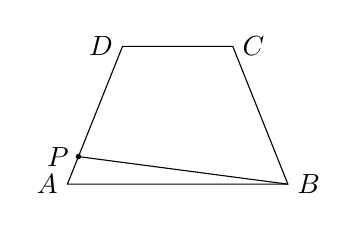
\begin{tikzpicture}[scale=0.7]
%\draw[help lines] (0,0) grid (4,4);
\draw (0,0) node[left](A){$A$} --(4,0)node[right](B){$B$} -- (3,2.5) node[right](C) {$C$}--(1,2.5) node[left](D){$D$}--cycle;
\coordinate[label=left:$P$] (P) at (0.2,0.5);
\draw[fill] (P) circle (1.1pt); 
\draw (P)--(4,0);
\end{tikzpicture}
\end{center}
		\qs 在平面直角坐标系$xOy$中,已知点$ A\left(\sqrt{3},0\right) ,~B\left(1,2\right)$,动点$P$满足$ \vv{OP}=\lambda\vv{OA}+\mu\vv{OB} $,其中$ \lambda ,~\mu\in\left[0,1\right] ,~\lambda+\mu\in\left[1,2\right]$,则所有点$ P $构成的图形面积为\xx
\onech{$ 1$}{$ 2$}{$ \sqrt{3}$}{$ 2\sqrt{3}$}
\qs
已知向量$ \vv{a},\vv{b} $满足$ |\vv{a} |=1,\vv{b}=(2,1)$,且$ \lambda \vv{a}+\vv{b}=\bm{0}~(\lambda\inR) $,则$ |\lambda |= $\tk.


\question
已知$A,B,C$是圆$O$上的三点,若$\vv{AO}=\dfrac{1}{2}\left(\vv{AB}+\vv{AC}\right)$,则$\vv{AB}$与$\vv{AC}$的夹角为\tk.
\qs 在四边形$ ABCD $中,$ AB=2 $.若$ \vv{DA}=\dfrac{1}{2}\left(\vv{CA}+\vv{CB}\right) $,则$ \vv{AB}\cdot\vv{DC}= $\tk.
\qs 已知两个单位向量$\vv{a}$,$\vv{b}$的夹角为$60^{\circ}$,$\vv{c}=t\vv{a}+(1-t)\vv{b}$,若$\xl{b}{c}=0$,则$t=$\tk.
\qs 若非零向量$ \bm{a,b} $满足$ \abs{\bm{a+b}}= \abs{\bm{a-b}}=\abs{\bm{2a}} $,则$ \bm{b} $与$ \bm{a+b} $的夹角是\tk.
\qs 在$\triangle ABC$中,$ O $为中线$ AM $上的一个动点,若$ AM=2 $,则$ \vv{OA}\bm{\cdot}\left(\vv{OB}+\vv{OC}\right) $的最小值是\tk.
\qs 平面向量$\bm{a}=\left(1,2\right),\bm{b}=\left(4,2\right),\bm{c}=m\bm{a}+\bm{b}\left(m\inR\right) $且$\bm{c} $与$ \bm{a} $的夹角等于$ \bm{c} $与$ \bm{b} $的夹角,则$ m= $\tk.
\qs 已知点$ P $在圆$ x^2+y^2=1 $上,点$ A $的坐标为$ (-2,0) $,$ O $为原点,则$ \vv{AO}\bm{\cdot}\vv{AP} $的最大值为\tk.

\qs 已知单位向量$ \bm{e}_1\text{与}\bm{e}_2 $的夹角为$ \alpha $,且$ \cos \alpha =\dfrac{1}{3},~$向量$ \bm{a}=3\bm{e}_1-2\bm{e}_2 $与$ \bm{b}=3\bm{e}_1-\bm{e}_2 $的夹角为$ \beta $,则$ \cos \beta =$\tk.
\qs 在三角形$\triangle ABC$中,点$ M,N $满足$ \vv{AM}=2\vv{MC} ,~$$ \vv{BN}=\vv{NC} .~$若$ \vv{MN}=x\vv{AB}+y\vv{AC} $,则$ x= $\tk;$~ y= $\tk.
\qs 已知点$ A(1,-1) ,B(3,0),C(2,1).$若平面区域$ D $由所有满足$ \vv{AP}=\lambda \vv{AB}+\mu \vv{AC}~(1\le \lambda \le 2,0\le \mu \le 1) $的点$ P $组成,则$ D $的面积为\tk.
\qs 已知$ O $为坐标原点,点$ P $为直线$ 2x+y-2=0 $上的任意一点,非零向量$ \bm{a}=(m,n) .$若$ \vv{OP}\bm{\cdot a} $恒为定值,则$ \dfrac{m}{n}= $\tk.
\qs 已知正方形$ ABCD $的边长为1,点$ E $是AB边上的动点,则$ \vv{DE}\cdot \vv{CB} $的值为\tk;~$ \vv{DE}\bm\cdot \vv{DC} $的最大值为\tk.

\qs 已知$ M $为$\triangle ABC$所在平面内的一点,且$ \vv{AM}=\dfrac{1}{4}\vv{AB}+n\vv{AC}. $若点$ M $在$\triangle ABC$内部(不含边界),则实数$ n $的取值范围是\tk. 
\qs 已知向量序列:$ \bm{a}_1,\bm{a}_2,\bm{a}_3,\cdots,\bm{a}_n,\cdots $满足如下条件:$ \left|\bm{a}_1\right|=4\left|\bm{d}\right|=2,~2\bm{a}_1\bm\cdot \bm{d}=-1 $且$ \bm{a}_n-\bm{a}_{n-1}=
\bm{d}~(n=,3,4,\cdots). $若$ \bm{a}_1\bm{\cdot}\bm{a}_k=0,~ $则$ k= $\tk;~$ \left|\bm{a}_1\right|,~  \left|\bm{a}_2\right|, \left|\bm{a}_3\right|,\cdots, \left|\bm{a}_n\right|,\cdots$中第\tk 项最小.
\qs 如图,$ \triangle AB_1C_1,~\triangle C_1B_2C_2,~\triangle C_2B_3C_3 $是三个边长为2的等边三角形,且有一条边在同一直线上,边$ B_3C_3 $上有两个不同的点$ P_1,~P_2,~ $则$ \vv{AB_2}\bm{\cdot}(\vv{AP_1}+\vv{AP_2}) =$\tk.
\begin{center}
\begin{tikzpicture}
%\draw[help lines](0,0) grid (6,2);
\tikzmath{
\a=sqrt(3);
}
\coordinate[label=below:$A$](A) at (0,0);
\foreach \p in {1,2,3}
\coordinate[label=below:$C_{\p}$] (C_\p) at($(\p*2,0)$) ;
\foreach \q in {1,2,3}
\coordinate[label=above:$B_{\q}$] (B_\q) at($(2*\q-1,\a)$);
\foreach \r in{1,2,3}
\draw (B_\r)--(C_\r);
\draw (A)--(C_3) (A)--(B_1) (C_1)--(B_2) (C_2)--(B_3);
\draw[->,>=stealth] (A)--(B_2) ;
\draw[->,>=stealth](A)--($(B_3)!0.3!(C_3)$) node[right](P_1){$P_1$};
\draw[->,>=stealth](A)--($(B_3)!0.7!(C_3)$) node[right](P_2){$P_2$};

\end{tikzpicture}
\end{center}

\qs 向量$ \vv{a},~\vv{b},\vv{c} $在正方形网格中的位置如图所示,若$ \vv{c}=\lambda\vv{a}+\mu\vv{b}~(\lambda,\mu \in \mathbf{R}) $,则$ \dfrac{\lambda}{\mu}=$\tk.
\begin{center}
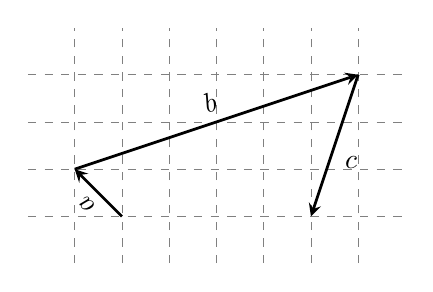
\begin{tikzpicture}[line width=1 pt,scale=0.6]
\draw[help lines,smooth, dashed] (-3.99,-2.99) grid (3.99,1.99);
\draw [->,>=stealth](-2,-2)--(-3,-1) node[sloped,midway,left,above,rotate=180](a){$\large\vv{a}$};
\draw [->,>=stealth](-3,-1)--(3,1) node[sloped,midway,left,above](b){$\large\vv{b}$};
\draw [->,>=stealth](3,1)--(2,-2) node[midway,below right ](c){$\large\vv{c}$};

\end{tikzpicture}
\end{center}
\qs 在$\triangle ABC$中,点$ M,N $满足$ \vv{AM}=2\vv{MC},~\vv{BN}=\vv{NC}. $若$ \vv{MN}=x\vv{AB}+y\vv{AC},~ $则$ x= $\tk;\\
$ y= $\tk.
\vspace{-2em}
\begin{center}
\begin{tikzpicture}
\draw(0,0)node[below](B){\small$B$}--(1,0)node[below](N){\small$N$}--(2,0)node[below](C){\small$C$};
\draw (0,0)--(1.1,2.1)node[above](A){\small$A$}--(2,0);
\draw (1,0)--(1.1,2.1);
\draw(1,0)--($(1.1,2.1)!0.7!(2,0)$)node[right](M){\small$M$};
\end{tikzpicture}
\end{center}

\qs 如图,在平行四边形$ ABCD $中,$ AP\bot BD~ $,垂足为$ P $,且$ AP=3 $,则$ \xl{AP}{AC}= $\tk.\begin{center}
\begin{tikzpicture}
%\draw[help lines](0,0) grid (4,4);
\coordinate [label=below:$B$](B) at(0,0);
\coordinate [label=below:$C$](C) at(3,0);
\coordinate [label=$A$](A) at(1,1.5);
\coordinate [label=$D$](D) at(4,1.5);
\draw (A)--(B)--(C)--(D)--cycle (A)--(C) (B)--(D);
\coordinate[label=below:$P$] (P) at($(B)!(A)!(D)$);
\draw (A)--(P);
\end{tikzpicture}
\end{center}
\vspace{-2em}
\qs 给定两个长度为$ 1 $的平面向量$ \vv{OA} $和$ \vv{OB} $,它们的夹角为$ 120^{\circ} $.如图所示,点$ C $在以$ O $为圆心的圆弧$ \wideparen{AB} $上变动,若$ \vv{OC}=x\vv{OA}+y\vv{OB} $,其中$ x,~y\inR $,则$ x+y $的最大值是\tk.
\begin{center}
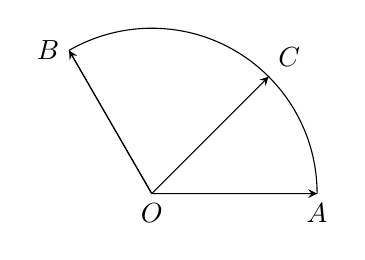
\begin{tikzpicture}[scale=0.7]
\coordinate[label=below:$O$](O) at(0,0);
\coordinate[label=below:$A$](A) at(0:3);
\coordinate[label=left:$B$](B) at(120:3);
\draw (O)--(A) (O)--(B);
\draw (3,0) arc (0:120:3);
\coordinate [label=above right:$C$](C) at(45:3);
\foreach \p in {A,B,C}
\draw[->,>=stealth](O)--(\p);
\end{tikzpicture}
\end{center}
\vspace{-2em}
\qs 如图,半径为$ \sqrt{3} $的扇形$ AOB $的圆心角为$ 120^{\circ} $,点$ C $在弧$ AB $上,且$ \angle COB=30^{\circ} $.若$ \vv{OC}=\lambda\vv{OA}+\mu\vv{OB} ,~$则$ \lambda+\mu= $\tk.
\begin{center}
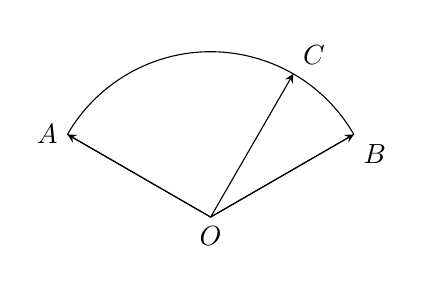
\begin{tikzpicture}[rotate=30,scale=0.7]
\coordinate[label=below:$O$](O) at(0,0);
\coordinate[label= below right:$B$](A) at(0:3);
\coordinate[label=left:$A$](B) at(120:3);
\draw (O)--(A) (O)--(B);
\draw (3,0) arc (0:120:3);
\coordinate [label=above right:$C$](C) at(30:3);
\foreach \p in {A,B,C}
\draw[->,>=stealth](O)--(\p);
\end{tikzpicture}
\end{center}
%\vspace{-2em}
\qs 在梯形$ ABCD $中,$ AB\sslash DC ,~AD\bot AB,AD=DC=\dfrac{1}{2}AB=2.$点$ N $是$ CD $边上的一动点,则$ \vv{AN}\bm{\cdot}\vv{AB} $的最大值为\tk.
\begin{center}
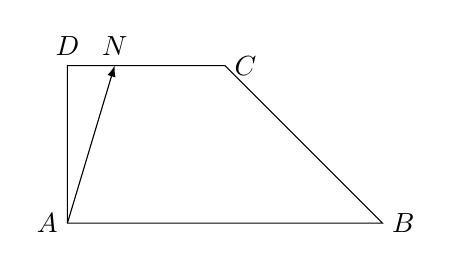
\begin{tikzpicture}
\coordinate[label=left:$A$] (A) at(0,0);
\coordinate[label=right:$B$] (B) at(4,0);
\coordinate[label=above:$D$] (D) at(0,2);
\coordinate [label=right:$C$](C) at(2,2);
\draw(A)--(B)--(C)--(D)--cycle;
\draw[->,>=latex](A)--(0.6,2) node[above](N) {$N$};
\end{tikzpicture}
\end{center}



\qs 如图,在直角梯形$ ABCD $中,$ AB\sslash CD,~AB\bot BC,~AB=2,~CD=1,~BC=a~(a>0),~ P$为线段$ AD $上一个动点,设$ \vv{AP}=x\vv{AD},~ \xl{PB}{PC}=y,~$对于函数$y=f(x),~$给出以下三个结论:\\
\ding{192} 当$ a=2 $时,函数$f(x)$的值域为$ \left[1,4\right] $;\\
\ding{193} $ \forall a\in\left(0,+\infty\right),~$都有$ f(1)=1 $成立;\\
\ding{194} $ \forall a\in\left(0,+\infty\right),~$函数$f(x)$的最大值都等于$ 4 $.\\
其中所有正确结论的序号是\tk.
\vspace{-7em}
\begin{flushright}
\begin{tikzpicture}[scale=1.2]
%\draw[help lines](0,0) grid (2.2,2.2);
\coordinate[label=below:$A$](A) at(0,0);
\coordinate[label=below:$B$](B) at(2,0);
\coordinate[label=left:$D$](D) at(1,2);
\coordinate[label=right:$C$](C) at(2,2);
\coordinate[label=left:$P$] (P) at($(A)!0.5!(D)$);
\draw (A)--(B)--(C)--(D)--cycle (B)--(P)--(C);
%\node(bq) at(2.1,0){$\text{图}1$};
\end{tikzpicture}
\end{flushright}

\end{questions}
\end{document}


